\documentclass{article}
\usepackage[utf8]{inputenc}
\usepackage{caption}
\usepackage{amsmath}
\usepackage{amssymb}
\usepackage{mathtools}
\usepackage{multicol}
\usepackage{graphicx}
\usepackage{wrapfig}
\usepackage{float}
\usepackage[makeroom]{cancel}
\usepackage{mhchem}

\graphicspath{ {../images/} }

\renewcommand{\baselinestretch}{1.5} % line spacing
\newcommand{\fline}{\par\noindent\rule{\textwidth}{0.1pt}} % horizontal line (wide)

\title{Unit 2 Kinetics\\Factors Affecting Rate of Reaction}
\author{Peter Zhang}

\begin{document}

\maketitle
\newpage
\tableofcontents
\newpage

% lesson 2

\section{Main Factors}
\begin{enumerate}
\item Temperature \begin{itemize} \item \ce{^ temp raises ^ in KE \\$\therefore$ ^ in collision frequency} \item \textbf{Helps} to overcome $E_{a}$ (activation energy) \item Many reacitons double in rate for every 10C \end{itemize}

\item Concentration \begin{itemize} \item \ce{^ Concentration, ^ rate increases} \item If more particles exist in the same amount of space, the likelihood of collisions happenning will be much higher \end{itemize}

\item Particle Size \begin{itemize} \item \ce{v in particle size, ^ in rate} \item by decreasing the size (particle surface area), there is more opportunity for higher reaction rate \item less energy required to move particles at same speed as bigger particles \item \textbf{By decreasing particle size} (similar to exploding dust filled room) increases reaction rate \end{itemize}

\item Pressure (Specific to Gasses) \begin{itemize} \item \ce{ ^ in pressure increases rate} \item \ce{more pressure means ^ collisions between gasses. Looking at Ideal Gas Laws... } \item Less volume for collisions results in more collisions \end{itemize}

\pagebreak

\item Catalyst \begin{itemize} \item \textbf{Only one that \underline{interferes} with $E_{a}$ (activation energy)} \item Equal for both forward and reverse reactions \item Catalysts \textbf{do not} change the yield \end{itemize} \begin{figure}[H] \centering 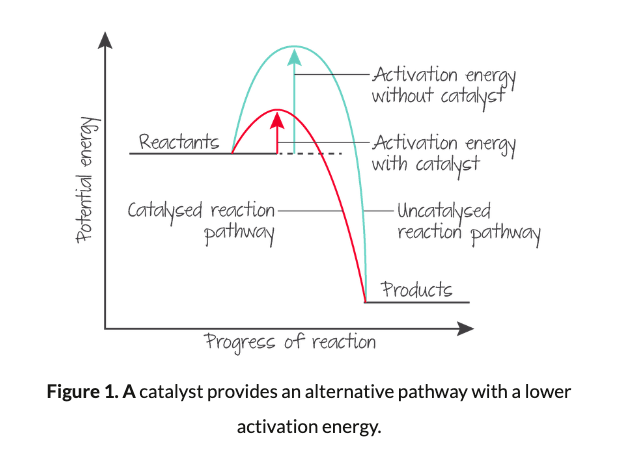
\includegraphics[width=\textwidth]{2.2fig1.png} \captionof{figure}{Catalysts and their effect on Activation Energy} \end{figure}

\end{enumerate}

\pagebreak

\section{Chart for Factor and Effect}

\begin{center}
	\begin{tabular}{|c|c|}
		\hline
		Factor & Effect \\
		\hline \hline
		Temperature Change & \ce{Temp ^ , Collision Frequency ^ | Temp v, Collision Frequency v} \\
		\hline
		Concentration Change & \ce{c ^ ,collision freq ^, c v, collision freq v}\\
		\hline 
		Particle SIze & \ce{Particle size v, collision rate ^}\\
		\hline
		Pressure (gas) & \ce{Pressure ^ , reaction rate ^}\\
		\hline
		Catalyst & LOWERS $E_{a}$ (Activation Energy)\\
		\hline
	\end{tabular}
\end{center}


\subsection{Sample Questions}

\subsection{Catalysts}
Catalytic converters used in cars reduce existence of harmful products such as \ce{CO(g) + NO(g) -> CO2(g) + 1/2 N2(g)}. Write an equation!

\ce{CO{g} + NO(g) ->[Pt\ or\ Rh] CO2(g) + 1/2 N2(g)}


\section{Rate Expressions}

$Reaction\ Rates = k_{\ce{[constant]}}(reactant)_{[reactant(s)\ concentration]}$

\subsection{Value for Reaction Rate}
Reaction Rate = $moldm^{-3} s^{-1}$

\subsection{Affecting Variables}
\ce{mA + nB -> products}\ where (m and n are coeffcients for reaction)

$$Rate\ \alpha\ k[A]^{m}[B]^{[n]}$$

Where m and n are coefficients and k is a constant.

\textbf{m and n} values from \textbf{experimental} is more \textbf{RELIABLE} than calculating it. The experimental process is much more accurate. 


\subsection{Sample Questions}

\begin{enumerate}

\item Calculate the value of k for the reaction of \ce{A + B -> products} if $[A] = 3.6*10^{-3}$ and $[B] = 2.2*10^{-2}$, $rate = 8.72*10^{-7}moldm^{-3}s^{-1}$ \begin{itemize} \item Rate equation: $k[A]^{3}[B]^{2}$ \begin{align*} k &= \frac{rate}{[A]^{3}[B]^{2}} \\ &= \frac{8.71*10^{-7}}{[3.6*10^{-3}][2.2*10^{-2}]}\\ &=38640mol^{-4}dm^{12}s{-1} \end{align*} \end{itemize}


\end{enumerate}








\end{document}